\section{Design}
This chapter describes the general design of Tsukiji.
We will discuss the architecture of the code base of Tsukiji and the dependencies that the program relies on.
For more detailed issues during the process of implementation, see section \ref{implementation}.

\subsection{Architecture}
Tsukiji consists of two main modules: orderbook and trader.
There are several smaller utility modules, the most important of these being the cryptography module.
How these modules interact is depicted in figure \ref{modulesfig}.
There are also several third-party libraries Tsukiji depends on.
The important ones are described later on in section \ref{dependencies}.

The trader module consists mainly of the Trader class.
Its main purpose is to communicate with other remote Traders.
The Trader class is a subclass of the DatagramProtocol class provided by the Twisted library \cite{twisted}.
This means the Trader class implements the UDP protocol.
The UDP protocol is the transport protocol used to talk to other traders.
UDP is chosen over TCP, because UDP travels more easily over NATs and firewalls.
This follows the design of Tribler and BitTorrent.
In section \ref{protocol} the application protocol is specified in detail.

The orderbook module has three main functionalities: 1. message creation for the application protocol and 2. managing the state of the orderbook itself and 3. matching bids and asks.
Message creation is used in combination with the trader module.
These are the messages that are passed around between peers.
Managing the state of the orderbook is an important task.
The orderbook keeps track of what offers come in, what offers are expired, or what trades have been made.
Finally, the matching algorithm is a simple algorithm.
For every new offer, incoming or outgoing, the algorithm checks whether there is an existing offer that matches with the new offer.
It tries to match favourable trades.
These functionalities are closely related, e.g. matching an ask with a bid produces a trade message, after which the orderbook is updated.

The cryptography module contains everything related to actions with public-key cryptography.
At the moment, it mostly functions as a wrapper around the PyCrypto library, for easier use within Tsukiji.
More on this can be read in section \ref{sprint1:identifiers}.

\begin{figure}[H]
  \centering
  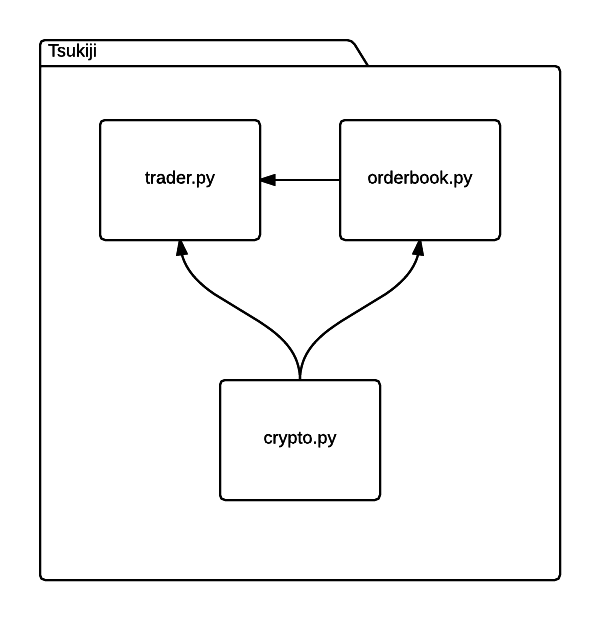
\includegraphics[width=\textwidth]{modules}
  \caption{A diagram with all of Tsukiji's modules}
  \label{modulesfig}
\end{figure}

\subsubsection{Dependencies}
\label{dependencies}
Tsukiji has two main third-party libraries it relies on: Twisted \cite{twisted} and PyCrypto \cite{pycrypto}.
Twisted is an open-source networking library.
It enjoys wide-spread use in the python world.
Tsukiji mainly makes use of its implementation of the UDP protocol.
For more information, see section \ref{sprint2:twisted}.

% PyCrypto
PyCrypto is a cryptography toolkit for python.
It comes with many functions related to cryptography, but we are mostly interested in functions related to public-key cryptography.
Each trader has a public/private key pair.
A trader's public key acts as their identifier.
For more information, see section \ref{sprint1:identifiers}.

